\newpage
\section{Photons and Their Quantum States in a Complex Vector Space}

\subsection*{From Numbers to Complex Vectors}

In classical computing, there are $\mathbb{N}\subset \mathbb{Z}\subset \mathbb{Q}\subset \mathbb{R}\subset \mathbb{C} $. 

Let $K$ be a field (域), which is a set (e.g., $\mathbb{R}$ or $\mathbb{C}$) where ordinary addition, substraction, multiplication and division are well-defined. A \hl{vector space} $V$ is a set where the addition of two vectors and a multiplication by an element of $K$ , so-called a scalar, are defined.

An element of $V = \mathbb{C}_n$ can be expressed as a column of $n$ complex numbers  $\chi_i (1 \le i \le n)$ as
\begin{align*}
    \ket{x}=\begin{pmatrix}
        \chi_1 \\ \vdots \\ \chi_n
    \end{pmatrix},\, \chi_i \in \mathbb{C}
\end{align*}


\subsection{Photon Polarization, an Example}
The polarization of a photon is an example of a two-dimensional complex vector space (i.e., a qubit). we can use a complex vector to represent an arbitrary polarization. The polarization of a photon can be measured by an analyzer, which allows the photon to pass with a probability.

\subsubsection{The Polarization of Light}
\begin{itemize}
    \item [\textbf{Property I}] Light is an electromagnetic wave. It is transverse, which means that the electric (and magnetic)  field of a light wave is perpendicular to the propagation direction. 
\end{itemize}

Recall that a planar and monochromatic scalar wave traveling in the $z$ direction has an amplitude of vibration
\begin{align*}
    u(z,t)=u_0\cos(kz-\omega t)
\end{align*}
where the speed of the wave $c=\frac{\omega}{k}$. 

At $z = 0$ (which can be generalized for arbitrary $z$), 
\begin{align*}
    u(t)\equiv u(z=0,t)=u_0 \cos\omega t
\end{align*}

For an electromagnetic wave, what oscillates is an $E$ vector in the $x -y$ plane (we ignore $B$ for simplicity).

\begin{itemize}
    \item [\textbf{Property II}]Light waves (with vector nature of $\vec{E}$ ) can be decomposed into two rays by birefringent crystals, such as Iceland spar.
\end{itemize}

\begin{figure}[H]
    \centering
    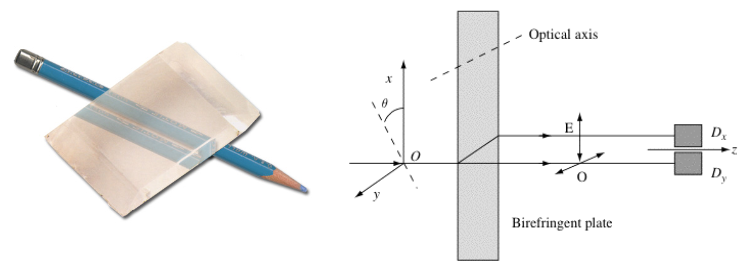
\includegraphics[width=0.44\textwidth]{QI2/Property II}
    \caption{Property II}
\end{figure}

For light with linear polarization
\begin{align*}
    E_x=& E_0\cos\theta\cos\omega t \\ 
    E_y=& E_0\sin\theta\cos\omega t
\end{align*}
So we can wirte
\begin{align*}
    \vec{E}=E_0 \hat{p} \cos\omega t,\,\hat{p}=(\cos\theta, \sin\theta)
\end{align*}

This can be achieved by letting light pass through a polarizer whose axis makes an angle $\theta$ with $x$ axis. The intensity of the light is proportional to the square electric field $I \propto E_0^2$. 

The Malus law $I'=I\cos^2\theta$.

In general, we have elliptical polarization
\begin{align*}
    E_x=& E_0\cos\theta\cos(\omega t-\delta_x)=E_0 Re\left( \mu e^{-i\omega t} \right) \\ 
    E_y=& E_0\sin\theta\cos(\omega t-\delta_y)=E_0 Re\left( \nu  e^{-i\omega t} \right)
\end{align*}
where $\mu=\cos\theta e^{i\delta_x}$ and $\nu=\sin\theta e^{i\delta_y}$, so $|\mu|^2+|\nu|^2=1$. It is important to note that only $\delta=\delta_y-\delta_x$ is physically relevant. This is because, by a time shift, we can choose $\delta_x=0$. 

Therefore, we can use a complex vector $\begin{pmatrix}
    \mu \\ \nu
\end{pmatrix}$ to represent an arbitrary polarization. The polarization vector is the same as $\begin{pmatrix}
    \mu e^{i\phi}\\ \nu e^{i\phi}
\end{pmatrix}$ for arbitrary $\phi$.

\subsubsection{The Quantum Interpretation}
Light is composed of photons, or light quanta. The Malus law now has a statistical interpretation, as photons cannot be further divided.

\subsection{Dirac’s Bracket Notation}
A complex vector space is composed of elements $\ket{a}$ called \hl{kets}. They are column vectors in our usual notation. It has a dual space whose elements are \hl{bras} $\bra{a}$. \hl{Inner product} $\braket{a|b}$ generalizes the dot product of usual vectors. Notice $\braket{a|b}=\braket{b|a}^{\dagger}$. Choosing an \hl{orthonormal basis} of kets $\ket{i}$ (notice $\braket{i|j}=\delta_{ij}$ ), we can expand an arbitrary ket $\ket{a}$ as
\begin{align*}
    \ket{a}=\sum_i\ket{i \braket{i|a}}
\end{align*}

\subsubsection{Vector Space in Quantum Mechanics}

In quantum mechanics, a vector space is composed of elements $\ket{a}$, known as \hl{kets} or ket-vectors (following Dirac’s invention). It satisfies the following axioms.
\begin{enumerate}
    \item The sum of any two kets is also a ket:
    \item Vector addition is commutative:
    \item Vector addition is associative:
    \item There is a unique vector 0 such that when you add it to any ket, it gives the same ket back:
    \begin{align*}
        \ket{a}+0=\ket{a}
    \end{align*}
    \item Given any ket $\ket{a}$, there is a unique $-\ket{a}$ such that: 
    \begin{align*}
        \ket{a}+(-\ket{a})=0
    \end{align*}
\end{enumerate}

The following two axioms involves the multiplication by any complex number. Ordinary vectors, however, can only be multiplied by real numbers.
\begin{enumerate}
    \item [(6)]Given any ket $\ket{a}$ and any complex number $\zeta $, you can multiply them to get a new ket. Also multiplication by a scalar is linear: 
    \begin{align*}
        \ket{a'}=\ket{\zeta a}=\zeta \ket{a}
    \end{align*}
    \item [(7)]The distributive property holds: 
    \begin{align*}
        \zeta(\ket{a}+\ket{b})=&\zeta\ket{a}+\zeta\ket{b}\\
        (\zeta+\omega)\ket{a}=&\zeta\ket{a}+\omega\ket{a}
    \end{align*}
\end{enumerate}


\subsubsection{The Complex Conjugate Vector Space}
A complex vector space has a dual space, i.e., the complex conjugate vector space.

For every ket $\ket{a}$, there is a \hl{bra} or bra-vector $\bra{a}$ in the dual space. Bras satisfy the same axiom as kets, with two notable differences:
\begin{itemize}
    \item Suppose $\bra{a}$ and $\bra{b}$ are the bras corresponding to the kets $\ket{a}$ and $\ket{b}$, respectively. Then the bra corresponding to $\ket{a} + \ket{b}$ is:
    \begin{align*}
        \bra{a}+\bra{b}
    \end{align*}
    \item The bra corresponding to $\zeta\ket{a}$ for any complex number $\zeta$ is
    \begin{align*}
        (\zeta\ket{a})^{\dagger}=\bra{a}\zeta^{\dagger}=\zeta^{\dagger}\bra{a}
    \end{align*}
\end{itemize}

\subsubsection{Inner Products}
The analog to the dot product for ordinary vectors is the \hl{inner product} for a bra and a ket is 〈b|a〉, which is a complex number.
\begin{itemize}
    \item The inner products are linear:
    \item Interchanging bras and kets corresponds to complex conjugation:
    \begin{align*}
        \braket{b|a}=\braket{a|b}^{\dagger}
    \end{align*}
    Hence, $\braket{a|a}$ is a real number. 
\end{itemize}

For example, if ket $\ket{a}$ and $\ket{b}$ are represented by the column vectors
\begin{align*}
    \ket{a}=\begin{pmatrix}
        \alpha_1 \\ \alpha_2\\ \alpha_3\\ \alpha_4 \\ \alpha_5
    \end{pmatrix},\, 
    \ket{b}=\begin{pmatrix}
        \beta_1 \\ \beta_2\\ \beta_3\\ \beta_4 \\ \beta_5
    \end{pmatrix}
\end{align*}
then the corresponding bra $\bra{b}$ is represented by the row vector
\begin{align*}
    \bra{b}=\begin{pmatrix}
        \beta_1^{\dagger}  & \beta_2^{\dagger} & \beta_3^{\dagger} & \beta_4^{\dagger}  & \beta_5^{\dagger}
    \end{pmatrix}
\end{align*}

The inner product is defined as the product of the row
vector and column vector:
\begin{align*}
    \braket{b|a}=&\begin{pmatrix}
        \beta_1^{\dagger}  & \beta_2^{\dagger} & \beta_3^{\dagger} & \beta_4^{\dagger}  & \beta_5^{\dagger}
    \end{pmatrix}\begin{pmatrix}
        \alpha_1 \\ \alpha_2\\ \alpha_3\\ \alpha_4 \\ \alpha_5
    \end{pmatrix}\\
    =& \beta_1^{\dagger} \alpha_1+ \beta_2^{\dagger}\alpha_2+ \beta_3^{\dagger}\alpha_3+ \beta_4^{\dagger} \alpha_4+ \beta_5^{\dagger}\alpha_5
\end{align*}

Observe that $\braket{b|a}=\braket{a|b}^{\dagger}$


\subsubsection{Normalized and Orthogonal Vectors}
Normalized vector is a generalization of unit vector in ordinary space. Normalized vectors satisfy
\begin{align*}
    \braket{a|a}=1
\end{align*}

In ordinary space, vectors are orthogonal if their dot product is zero (they are also said to be perpendicular to each other). In Hilbert space, two vectors are orthogonal if
\begin{align*}
    \braket{b|a}=0
\end{align*}

\subsubsection{Basis and Basis Vectors}
Let us consider a set of $k$ vectors $\left\{ \ket{x_1}, \dots,\ket{x_k} \right\}$ in $V = \mathbb{C}_n$. The set is said to be linearly dependent if the equation
\begin{align*}
    \sum_{i=1}^k \eta_i \ket{x_i}=\ket{0} 
\end{align*}
has a solution $\eta_1,\dots,\eta_k$ , at least one of which is non-vanishing. 

If the trivial solution $\eta_i = 0 (1 \le i \le k)$ is the only solution, the set is said to be \hl{linearly independent}.

The set of n linearly independent vectors is called a \hl{basis} of $\mathbb{C}_n$ and the vectors are called \hl{basis vectors}. 

\subsubsection{Orthonormal Basis and Completeness}

Any vector $\ket{a}$ can be written as a sum of basis
\begin{align*}
    \ket{a}=\sum_i \alpha_i \ket{i}
\end{align*}
where the complex number $\alpha_i$ are called the components of the vector.

We can calculate an individual component corresponding to the basis vector $\ket{j}$ as
\begin{align*}
    \alpha_j=\braket{j|a}
\end{align*}
since $\braket{j|i}=\delta_{ij}$ (i.e. 1 if $i=j$ else 0). 

Therefore, we can also rewrite the decomposition of the vector $\ket{a}$ in a more elegant form as
\begin{align*}
    \ket{a}=\sum_i \ket{i} \braket{i|a}
\end{align*}
which implies the following identity:
\begin{align*}
    \sum_i \ket{i}\bra{i}=I
\end{align*}
where $I$ is an identity operator $\begin{pmatrix}
    1 & 0 \\ 0 & 1
\end{pmatrix}$ (note that we will come back to the definition of operator).

\subsubsection{Projection Operators}
The matrix
\begin{align*}
    P_k=\ket{k}\bra{k}
\end{align*}
introduced above is called a \hl{projection operator (投影算符)} in the direction defined by $\ket{k}$. This projects a vector $\ket{v}$ to a vector parallel to $\ket{k}$ in such a way that $\ket{v}-P_k\ket{v}$ is orthogonal to $\ket{k}$. 

The set $\left\{ P_k=\ket{k}\bra{k} \right\}$ satisfies the conditions
\begin{enumerate}
    \item $\displaystyle P_k^2=P_k$
    \item $\displaystyle P_kP_j=0 \, (k \ne j)$
    \item $ \displaystyle \sum_k P_k =I$ (completeness relation)
\end{enumerate}

\subsection{Photon Polarization in the New Language}
Photon polarization lives in a 2D complex vector space. An orthonormal basis can be chosen to be linear polarization along x and y axes.
\begin{align*}
    \ket{h}=\begin{pmatrix}
        1\\0
    \end{pmatrix},\, \ket{v}=\begin{pmatrix}
        0\\1
    \end{pmatrix}
\end{align*}

The corresponding projection operators are
\begin{align*}
    P_h=\ket{h}\bra{h}=\begin{pmatrix}
        1 & 0\\ 0 & 0
    \end{pmatrix}, \, P_v=\ket{v}\bra{v}=\begin{pmatrix}
        0 & 0\\ 0 & 1
    \end{pmatrix}
\end{align*}
We confirm the completeness condition $P_h+P_v=I_{2\times 2}$

A general state $\ket{p}$ of a photon is represented by a unit vector
\begin{align*}
    \ket{p}=I\ket{p}=\ket{h}\braket{h|p}+\ket{v}\braket{v|p}=\mu\ket{h}+\nu\ket{v}
\end{align*}
where $\mu,\nu \in \mathbb{C}$ and $\braket{p|p}=|\mu|^2+|\nu|^2=1$

The components of $\ket{p}$, 
\begin{align*}
    \mu=\braket{h|p},\, \nu =\braket{v|p}
\end{align*}
are known as the \hl{probability amplitudes}.

The probabilities for the measurements of horizontal and vertical polarizations are given by
\begin{align*}
    P_h=& |\mu|^2=\braket{p|h}\braket{h|p}\equiv \braket{p | P_h | p} \\
    P_v=& |\nu|^2=\braket{p|v}\braket{v|p}\equiv \braket{p | P_v | p}
\end{align*}

The total probability $P_h+P_v=1$. After the measurement, the photon is either in the state $\ket{h}$ or in the state $\ket{v}$.